\documentclass[aspectratio=169, 10pt]{beamer}

% --- PACKAGES ---
\usepackage[utf8]{inputenc}
\usepackage{tikz}
\usetikzlibrary{shapes.geometric, arrows.meta, positioning, calc}
\usepackage{booktabs}
\usepackage{array}
\usepackage{xcolor}

% --- COLOR PALETTE ---
\definecolor{Ink}{HTML}{1A1D23}
\definecolor{Dim}{HTML}{6B7280}
\definecolor{Accent}{HTML}{2C5F8A}
\definecolor{AccentSoft}{HTML}{EFF3F7}
\definecolor{Line}{HTML}{D8DCE2}
\definecolor{Warn}{HTML}{9A4B3C}
\definecolor{TealAccent}{HTML}{2C5F8A}
\definecolor{AmberAccent}{HTML}{D97706}
\definecolor{CardBg}{HTML}{F8FAFC}
\definecolor{TextDim}{HTML}{6B7280}

% --- BEAMER THEME CUSTOMIZATION ---
\setbeamercolor{background canvas}{bg=white}
\setbeamercolor{normal text}{fg=Ink}
\setbeamercolor{title}{fg=Ink}
\setbeamercolor{subtitle}{fg=Dim}
\setbeamercolor{author}{fg=Dim}
\setbeamercolor{date}{fg=Dim}
\setbeamercolor{item}{fg=Accent}
\setbeamercolor{subitem}{fg=Dim}
\setbeamercolor{block title}{bg=AccentSoft, fg=Accent}
\setbeamercolor{block body}{bg=white, fg=Ink}
\setbeamertemplate{itemize items}[circle]
\setbeamertemplate{navigation symbols}{}
\setbeamertemplate{blocks}[rounded][shadow=false]
\setlength{\parskip}{0pt}

% Safer frametitle template: works with or without frame subtitles.
\setbeamertemplate{frametitle}{
  \vspace{0.25cm}
  {\large\bfseries\color{Ink}\insertframetitle\par}
  \ifx\insertframesubtitle\empty
  \else
    \vspace{1pt}
    {\footnotesize\color{Dim}\insertframesubtitle\par}
  \fi
  \vspace{3pt}
  {\color{Line}\rule{\linewidth}{0.6pt}\par}
  \vspace{4pt}
}

\setbeamertemplate{footline}{
  \hfill\raisebox{6pt}{\color{Dim}\scriptsize\insertframenumber\,/\,\inserttotalframenumber}\hspace{8pt}\vspace{2pt}
}

\setbeamertemplate{title page}{
  \vspace{2.2cm}
  {\color{Line}\rule{\linewidth}{0.6pt}}\\[0.5cm]
  {\centering\Huge\bfseries\color{Ink}\inserttitle\par}
  \vspace{0.25cm}
  {\centering\large\color{Accent}\insertsubtitle\par}
  \vspace{0.6cm}
  {\centering\normalsize\color{Dim}\insertauthor\par}
  \vspace{0.15cm}
  {\centering\normalsize\color{Dim}\insertdate\par}
  \vspace{0.4cm}
  {\color{Line}\rule{\linewidth}{0.6pt}}
}

% --- METADATA ---
\title{VANGUARD}
\subtitle{Autonomous Smart Perimeter Monitoring \& Warning Platform}
\author{ATmega32-Based Embedded Systems Design \\ Student ID: 2205139, 2205143, 2205147}
\date{Project Proposal}

\begin{document}

% --- SLIDE 1: TITLE ---
\begin{frame}
    \titlepage
\end{frame}

% --- SLIDE 2: MOTIVATION - PROBLEM DESCRIPTION & IMPORTANCE ---
\begin{frame}{1. Motivation}{Problem Description \& Importance}
    \begin{columns}[T]
        \begin{column}{0.48\textwidth}
            \begin{block}{Problem Description}
                \small
                \begin{itemize}
                    \item Conventional perimeter systems often rely on a single trigger source such as PIR or optical tripwire sensing.
                    \item False alarms can occur because of wind, foliage, small animals, and environmental disturbances.
                    \item Passive systems cannot aim toward the triggered sector or locally verify whether a warm object is present.
                \end{itemize}
            \end{block}
        \end{column}
        \begin{column}{0.48\textwidth}
            \begin{block}{Why It Matters}
                \small
                \begin{itemize}
                    \item Remote sites, industrial zones, and restricted areas need fast local detection without depending fully on human response time.
                    \item Combining motion, distance, heat, and badge authentication reduces false alarms.
                    \item A staged verification pipeline is safer than directly acting on a single sensor trigger.
                \end{itemize}
            \end{block}
        \end{column}
    \end{columns}
\end{frame}

% --- SLIDE 3: MOTIVATION - WHY THIS PROJECT & OBJECTIVES ---
\begin{frame}{1. Motivation}{Why This Project \& Main Objectives}
    \footnotesize The project integrates static-sector sensing, hardware-PWM servo positioning, multi-bus communication, and interrupt-driven control on the ATmega32. The aim is a complete embedded prototype, not an isolated sensor demo.
    \vspace{0.05cm}
    \begin{enumerate}
        \footnotesize
        \item \textbf{Static-sector PIR detection:} three fixed PIR sensors (INT0/INT1/INT2) each watch a static $\approx$60$^\circ$ sector across the 180$^\circ$ field; the turret does not mechanically sweep, so a moving platform never crosses its own static thermal background.
        \item \textbf{Precision lock-on:} a sector trigger slews the pan servo to that sector's center (worst case 60$^\circ$ from the centered idle position), then a $\pm 10$--15$^\circ$ horizontal micro-scan and vertical elevation micro-scan run concurrently on independent PWM channels (OC1A/OC1B) to center the narrow VL53L0X beam on the target within $\approx$650 ms.
        \item \textbf{Multi-modal verification:} thermal $\Delta T$ using MLX90614 and distance $R$ using VL53L0X over I$^2$C.
        \item \textbf{Wireless IFF handshake:} application-layer RF badge challenge-response over SPI using nRF24L01+, with a rolling counter/nonce in each payload to reject replayed transmissions.
        \item \textbf{Warning actuator:} MOSFET-driven strobe/alarm output after failed authorization and positive sensor verification.
        \item \textbf{Stretch features:} UART monitoring dashboard and optional MicroSD incident logging.
    \end{enumerate}
\end{frame}

% --- SLIDE 3B: MOTIVATION - REAL-WORLD DEPLOYMENT SCENARIOS ---
\begin{frame}{1. Motivation}{Real-World Deployment Scenarios}
    \tiny
    \begin{table}
        \centering
        \begin{tabular}{p{2.7cm} p{3.0cm} p{5.3cm}}
            \toprule
            \textbf{\color{Accent} Operational Sector} & \textbf{\color{Accent} Threat Profile} & \textbf{\color{Accent} After Sector PIR Trigger + Slew} \\
            \midrule
            Remote substation / solar farm perimeter & Night intrusion, cable theft, wildlife false alarms & VERIFY confirms human presence, silently reverts to SECTOR WATCH on animals/wind $\rightarrow$ IFF fails (unbadged) $\rightarrow$ strobe + incident log \\
            Restricted depot (munitions, server vault) & Unauthorized entry, tailgating behind a badged employee & LOCK-ON micro-scan counts ToF clusters $\rightarrow$ slotted IFF window $\rightarrow$ badges $<$ targets $\rightarrow$ alarm + escort-breach log \\
            Automated hazard cell (robotic/welding bay) & Personnel entering an active machinery envelope & LOCK-ON + VERIFY confirm presence $\rightarrow$ IFF fails (no badges provisioned for an active zone) $\rightarrow$ interlock trip \\
            \bottomrule
        \end{tabular}
    \end{table}
    \vspace{0.1cm}
    {\tiny\color{TextDim} All three share the same unmodified FSM (Section 4: Role of the ATmega32) -- only badge provisioning and operator response differ by deployment.}
    \vspace{0.1cm}
    \footnotesize
    \begin{itemize}
        \item \textbf{Remote infrastructure watch:} multi-modal VERIFY (heat + range) filters out the wildlife/foliage false alarms that dominate single-sensor tripwires, without needing a manned response for every trigger.
        \item \textbf{Escort-aware access control:} the same micro-scan used for azimuth refinement doubles as a target counter, catching a side-by-side companion that a badge-only IFF check would miss; a target fully hidden directly behind another remains a known limitation of a single-beam ToF scan.
        \item \textbf{Industrial safety interlock:} no badges are provisioned for an active hazard zone, so any VERIFY-confirmed presence reaches WARNING OUTPUT through the same FSM; the MOSFET drives a safety relay directly, with no PC/network round-trip in the path.
    \end{itemize}
\end{frame}

% --- SLIDE 4: EQUIPMENT - COMPONENT TABLE ---
\begin{frame}{2. Equipment}{Hardware Components \& Justification}
    \tiny
    \renewcommand{\arraystretch}{0.93}
    \begin{table}
        \centering
        \begin{tabular}{p{2.15cm} p{2.85cm} p{5.6cm}}
            \toprule
            \textbf{\color{Accent} Purpose} & \textbf{\color{Accent} Exact Module Used} & \textbf{\color{Accent} Justification} \\
            \midrule
            System Controller & ATmega32-16PU & On-chip TWI, SPI, USART, timers, interrupts, and GPIO support the complete prototype without external bus bridges. \\
            Motion Detection & 3$\times$ PIR Motion Sensor (fixed, sector-mounted) & Fixed at $\approx$30$^\circ$/90$^\circ$/150$^\circ$ sector centers, not on the moving head, so panning never sweeps the sensor's FOV across its own thermal background; edges on INT0/INT1/INT2 each command a slew to that sector. \\
            Thermal Verification & MLX90614 IR Sensor & Factory-calibrated non-contact temperature reading over I$^2$C; useful for warm-object verification. \\
            Distance Measurement & VL53L0X Laser ToF & Digital laser time-of-flight ranging over I$^2$C; less affected by air temperature and wind than ultrasonic ranging; driven with a minimal bare-metal register driver rather than the full ST API to conserve Flash. \\
            Wireless IFF Link & nRF24L01+ Pair & Low-latency 2.4 GHz packet radio over SPI for challenge-response badge authentication. \\
            Black-Box Logging & MicroSD Card Module & Optional high-capacity non-volatile storage over SPI for incident event logs, written via Petit FatFs / raw 512 B block writes rather than full FatFs to minimize SRAM use. \\
            Pan-Tilt Actuation & MG996R Servos ($\times$2) & Standard hobby servo interface; driven by Timer1 50 Hz PWM outputs OC1A and OC1B. \\
            Telemetry Bridge & FTDI FT232RL & Bridges ATmega32 USART to a PC USB port for the optional monitoring dashboard. \\
            Warning Output & MOSFET + Strobe/Alarm & Low-side switch driven by GPIO to safely control a higher-current warning actuator, with a flyback diode across the inductive load to clamp switch-off voltage spikes. \\
            Power Regulation & Dual LM2596 Converters & Two dedicated channels: one for the 5 V logic rail, one strictly for 6 V servo power, plus a Schottky diode isolating the logic rail from servo-switching transients; pan/tilt slews are staggered (never simultaneous max-torque) to stay under the servo channel's 3.5 A rating despite a $\approx$5 A combined MG996R stall current, backed by a 1000 $\mu$F bulk cap. \\
            Level Compatibility & 3.3 V Regulator / Level Shifter & Protects 3.3 V modules such as VL53L0X and nRF24L01+ when used with a 5 V ATmega32 system. \\
            \bottomrule
        \end{tabular}
    \end{table}
\end{frame}

% --- SLIDE 5: EQUIPMENT - ALTERNATIVES COMPARISON ---
\begin{frame}{2. Equipment}{Comparison with Simpler Alternatives}
    \tiny
    \begin{table}
        \centering
        \begin{tabular}{p{1.8cm} p{2.35cm} p{2.45cm} p{4.1cm}}
            \toprule
            \textbf{\color{Accent} Subsystem} & \textbf{\color{Accent} Selected Module} & \textbf{\color{Accent} Simpler Alternative} & \textbf{\color{Accent} Why We Chose Selected Over Alternative} \\
            \midrule
            Distance & VL53L0X Laser ToF & HC-SR04 Ultrasonic & Laser ToF gives compact digital ranging and is less affected by air temperature/wind than sound-based ranging. \\
            Thermal & MLX90614 IR Sensor & LM35 Temperature Sensor & LM35 requires contact; MLX90614 supports non-contact warm-target verification. \\
            Wireless & nRF24L01+ RF & HC-05 Bluetooth Module & nRF24L01+ supports fast packet-based custom challenge-response logic without Bluetooth pairing delay. \\
            Logging & MicroSD Card & SPI EEPROM & MicroSD provides much larger storage for optional incident logs. \\
            Controller & ATmega32-16PU & Arduino Uno Board & ATmega32 gives direct DIP-40 pin access and encourages register-level peripheral design. \\
            \bottomrule
        \end{tabular}
    \end{table}
\end{frame}

% --- SLIDE 6: EQUIPMENT - SOFTWARE ---
\begin{frame}{2. Equipment}{Software \& Development Tools}
    \begin{columns}[T]
        \begin{column}{0.5\textwidth}
            \begin{block}{Toolchain}
                \small
                \begin{itemize}
                    \item \textbf{Microchip Studio / AVR-GCC} -- C development, register-level drivers, compilation
                    \item \textbf{USBasp / eXtreme Burner} -- firmware flashing
                    \item \textbf{Proteus VSM} -- circuit simulation before fabrication
                \end{itemize}
            \end{block}
        \end{column}
        \begin{column}{0.5\textwidth}
            \begin{block}{Host-Side Tools}
                \small
                \begin{itemize}
                    \item \textbf{Python 3 (PySerial)} -- UART telemetry parsing
                    \item \textbf{Pygame / Tkinter} -- radar-style monitoring dashboard
                \end{itemize}
            \end{block}
        \end{column}
    \end{columns}
    \vspace{0.2cm}
    \footnotesize\color{Dim} The ATmega32 performs sensing, verification, aiming, and warning control autonomously. The PC dashboard is only a visualization and debugging tool.
\end{frame}

% --- SLIDE 7: SYSTEM DESIGN - BLOCK DIAGRAM ---
\begin{frame}{3. System Design}{System Block Diagram}
    \centering
    \resizebox{0.98\textwidth}{!}{
        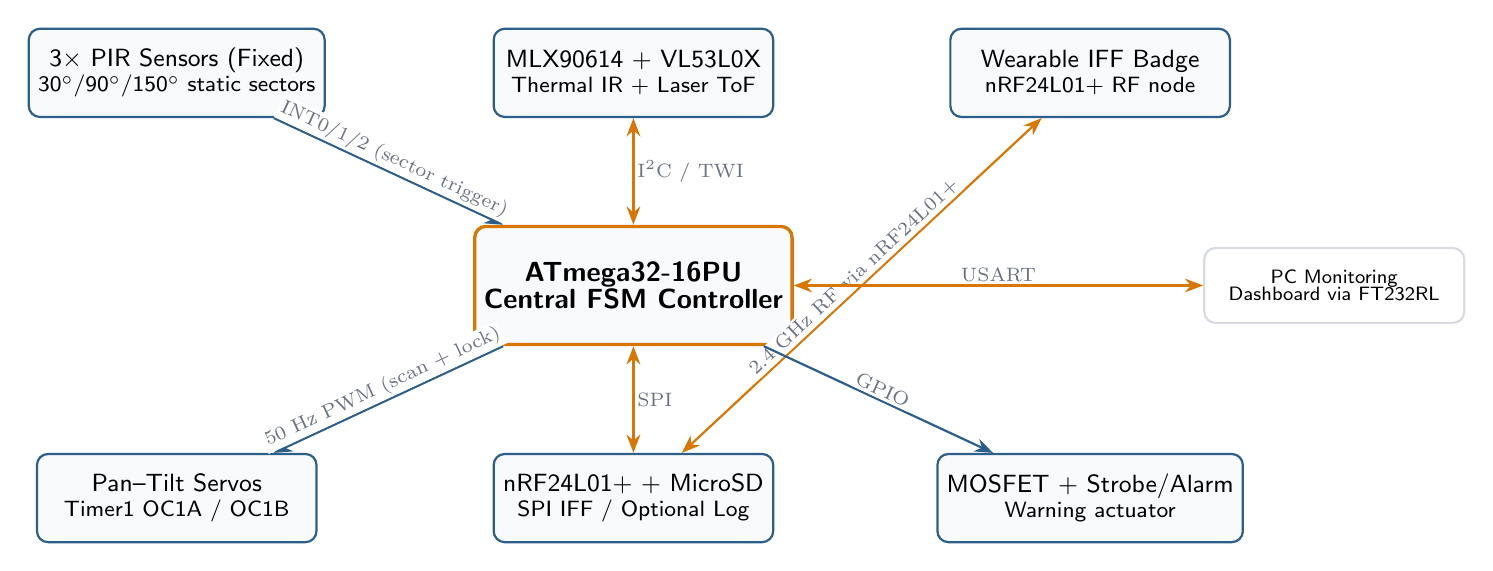
\begin{tikzpicture}[
            mcu/.style={rectangle, draw=AmberAccent, very thick, fill=CardBg, rounded corners, minimum height=1.5cm, minimum width=3.8cm, align=center, font=\sffamily\bfseries\normalsize},
            block/.style={rectangle, draw=TealAccent, thick, fill=CardBg, rounded corners, minimum height=1.12cm, minimum width=3.55cm, align=center, font=\sffamily\small},
            smallblock/.style={rectangle, draw=Line, thick, fill=white, rounded corners, minimum height=0.95cm, minimum width=3.3cm, align=center, font=\sffamily\scriptsize},
            arrow/.style={-Stealth, thick, color=TealAccent},
            biarrow/.style={Stealth-Stealth, thick, color=AmberAccent},
            lbl/.style={font=\scriptsize, color=TextDim, fill=white, inner sep=1pt}
        ]
            % Sensing layer
            \node[block] (pir) at (-5.8,2.7) {3$\times$ PIR Sensors (Fixed)\\[-2pt]\footnotesize 30$^\circ$/90$^\circ$/150$^\circ$ static sectors};
            \node[block] (thermal) at (0,2.7) {MLX90614 + VL53L0X\\[-2pt]\footnotesize Thermal IR + Laser ToF};
            \node[block] (badge) at (5.8,2.7) {Wearable IFF Badge\\[-2pt]\footnotesize nRF24L01+ RF node};

            % Central controller
            \node[mcu] (mcu) at (0,0) {ATmega32-16PU\\[-2pt]\normalsize Central FSM Controller};

            % Output layer
            \node[block] (servo) at (-5.8,-2.7) {Pan--Tilt Servos\\[-2pt]\footnotesize Timer1 OC1A / OC1B};
            \node[block] (wireless) at (0,-2.7) {nRF24L01+ + MicroSD\\[-2pt]\footnotesize SPI IFF / Optional Log};
            \node[block] (warning) at (5.8,-2.7) {MOSFET + Strobe/Alarm\\[-2pt]\footnotesize Warning actuator};

            % Optional PC
            \node[smallblock] (pc) at (8.9,0) {PC Monitoring\\[-2pt] Dashboard via FT232RL};

            % Connections
            \draw[arrow] (pir) -- node[lbl, above, sloped]{INT0/1/2 (sector trigger)} (mcu);
            \draw[biarrow] (thermal) -- node[lbl, right]{I$^2$C / TWI} (mcu);
            \draw[biarrow] (badge) -- node[lbl, above, sloped]{2.4 GHz RF via nRF24L01+} (wireless);
            \draw[arrow] (mcu) -- node[lbl, above, sloped]{50 Hz PWM (scan + lock)} (servo);
            \draw[biarrow] (mcu) -- node[lbl, right]{SPI} (wireless);
            \draw[arrow] (mcu) -- node[lbl, above, sloped]{GPIO} (warning);
            \draw[biarrow] (mcu) -- node[lbl, above]{USART} (pc);
        \end{tikzpicture}
    }
    \vspace{0.1cm}

    {\tiny\color{TextDim} $\rightarrow$ one-way control/signal path \quad $\leftrightarrow$ bidirectional/shared communication path.}
\end{frame}

% --- SLIDE 8: SYSTEM DESIGN - PINOUT MAP ---
\begin{frame}{3. System Design}{ATmega32 Interface Pinout Allocation Map}
    \scriptsize
    \renewcommand{\arraystretch}{0.92}
    \begin{table}
        \centering
        \begin{tabular}{lll}
            \toprule
            \textbf{\color{Accent} Pin(s)} & \textbf{\color{Accent} Function} & \textbf{\color{Accent} Connected To} \\
            \midrule
            PD0 (RXD), PD1 (TXD) & Hardware USART & FTDI FT232RL, 115200 baud \\
            PD2 (INT0) & External interrupt 0 & Fixed sector PIR 1 ($\approx$30$^\circ$); commands servo slew to sector center \\
            PD3 (INT1) & External interrupt 1 & Fixed sector PIR 2 ($\approx$90$^\circ$); commands servo slew to sector center \\
            PB2 (INT2) & External interrupt 2 & Fixed sector PIR 3 ($\approx$150$^\circ$); commands servo slew to sector center \\
            PD5 (OC1A) & Timer1 hardware PWM & Pan servo control signal \\
            PD4 (OC1B) & Timer1 hardware PWM & Tilt servo control signal \\
            PC0 (SCL), PC1 (SDA) & Hardware TWI (I$^2$C) & MLX90614 and VL53L0X, 7-bit addresses 0x5A and 0x29 \\
            PB5/PB6/PB7 & Hardware SPI & MOSI / MISO / SCK for nRF24L01+ and MicroSD \\
            PB4 (SS) & SPI master safety pin & Configure as output and keep HIGH \\
            PA1 & GPIO output & MicroSD chip select (CS\_SD) \\
            PA2 & GPIO output & nRF24L01+ CSN \\
            PA3 & GPIO output & nRF24L01+ CE \\
            PA4 & GPIO input, optional & nRF24L01+ IRQ \\
            PD6 & GPIO output & Warning strobe/alarm MOSFET gate \\
            \bottomrule
        \end{tabular}
    \end{table}
\end{frame}

% --- SLIDE 9: ROLE OF THE ATMEGA32 - FSM ---
\begin{frame}{4. Role of the ATmega32}{Finite State Machine Logic}
    \centering
    \vspace{0.02cm}
    \resizebox{0.72\textwidth}{!}{
        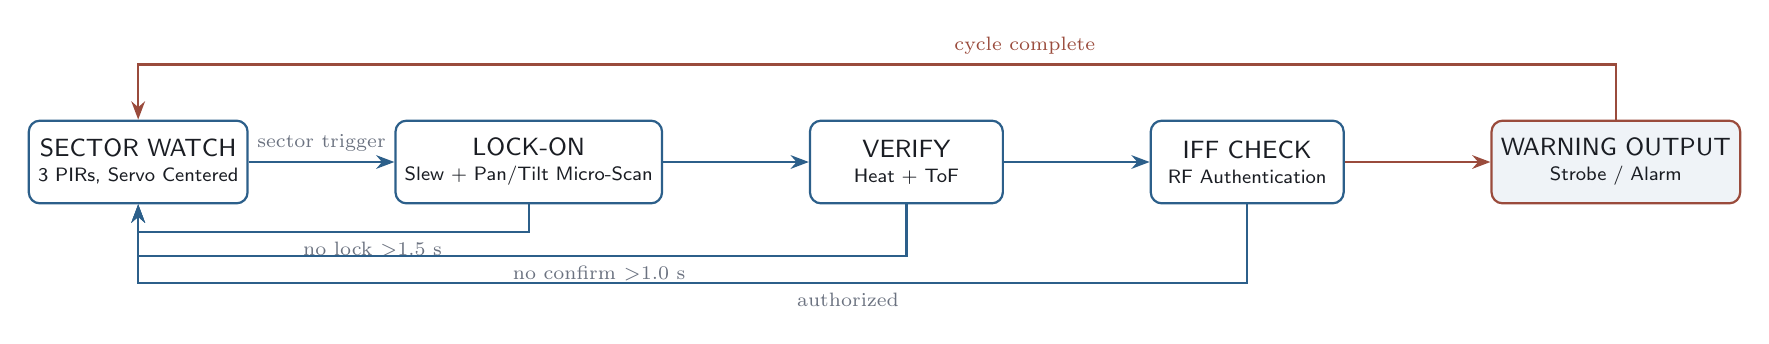
\begin{tikzpicture}[
            node distance=1.85cm,
            state/.style={
                rectangle,
                draw=Accent,
                fill=white,
                thick,
                rounded corners,
                minimum height=1.05cm,
                minimum width=2.45cm,
                align=center,
                font=\sffamily\small,
                text=Ink
            },
            alertstate/.style={
                state,
                draw=Warn,
                fill=AccentSoft
            },
            arrow/.style={-Stealth, thick, color=Accent},
            alertarrow/.style={-Stealth, thick, color=Warn},
            note/.style={font=\scriptsize, color=Dim}
        ]
            \node[state] (scan) {SECTOR WATCH\\[-2pt]\scriptsize 3 PIRs, Servo Centered};
            \node[state, right=of scan] (lock) {LOCK-ON\\[-2pt]\scriptsize Slew + Pan/Tilt Micro-Scan};
            \node[state, right=of lock] (verify) {VERIFY\\[-2pt]\scriptsize Heat + ToF};
            \node[state, right=of verify] (iff) {IFF CHECK\\[-2pt]\scriptsize RF Authentication};
            \node[alertstate, right=of iff] (warn) {WARNING OUTPUT\\[-2pt]\scriptsize Strobe / Alarm};

            % Main forward flow
            \draw[arrow] (scan) -- node[above, note]{sector trigger} (lock);
            \draw[arrow] (lock) -- (verify);
            \draw[arrow] (verify) -- (iff);
            \draw[alertarrow] (iff) -- (warn);

            % Feedback / return paths
            \draw[arrow] (lock.south) -- ++(0,-0.35) -| node[pos=0.20, below, note]{no lock $>$1.5 s} (scan.south);
            \draw[arrow] (verify.south) -- ++(0,-0.65) -| node[pos=0.20, below, note]{no confirm $>$1.0 s} (scan.south);
            \draw[arrow] (iff.south) -- ++(0,-1.00) -| node[pos=0.18, below, note]{authorized} (scan.south);
            \draw[alertarrow] (warn.north) -- ++(0,0.70) -| node[pos=0.20, above, note, text=Warn]{cycle complete} (scan.north);
        \end{tikzpicture}
    }

    \vspace{0.08cm}
    \begin{itemize}
        \footnotesize
        \item Three fixed PIR sensors (INT0/INT1/INT2) each watch a static $\approx$60$^\circ$ sector; the turret stays centered and does not mechanically sweep, so it never crosses its own thermal background.
        \item On a sector trigger, the pan servo slews to that sector's center (worst case 60$^\circ$, $\approx$250 ms at the MG996R's loaded $\approx$0.2 s/60$^\circ$ rate); \textbf{LOCK-ON} then runs the horizontal and vertical micro-scans concurrently on independent PWM channels, for $\approx$650 ms total; no return within \textbf{1.5 s} reverts to \textbf{SECTOR WATCH}.
        \item \textbf{VERIFY} confirms agreeing heat + range readings and counts distinct ToF depth clusters from the micro-scan; \textbf{IFF CHECK} cross-checks that count against slotted badge responses (Badge\_ID $\times$ 4 ms + random backoff, 40 ms RX window) to flag piggybacking, or reverts within \textbf{1.0 s}.
        \item Further feedback paths return to \textbf{SECTOR WATCH} once the IFF is authorized or the warning cycle completes.
        \item \textbf{Fail-safe degraded modes:} SCL held low $>$10 ms triggers a software TWI bus-reset (toggle SCL up to 9 times); an unresponsive nRF24 radio falls back to a stricter High-Alert VERIFY (double ToF check + extended $\Delta T$ hold) before WARNING OUTPUT.
    \end{itemize}
\end{frame}

% --- SLIDE 10: ROLE OF THE ATMEGA32 - PERIPHERAL UTILIZATION ---
\begin{frame}{4. Role of the ATmega32}{Peripheral Utilization Breakdown}
    \footnotesize
    \begin{itemize}
        \item \textbf{GPIO:} warning MOSFET control, status indicators, SPI chip-select/control lines.
        \item \textbf{External interrupts (INT0/INT1/INT2):} low-latency edge triggers from three fixed sector PIRs; each is masked during LOCK-ON/VERIFY and re-armed only after its line returns low in SECTOR WATCH, to guard against the sensor's 2.5--5 s output hold time.
        \item \textbf{Timer1 (16-bit):} exact 50 Hz servo PWM using OC1A and OC1B for pan and tilt.
        \item \textbf{Timer0:} 1 ms system tick for non-blocking task scheduling and state-machine timing.
        \item \textbf{Timer2:} spare timer, reserved headroom for additional timeout generation as the FSM is extended.
        \item \textbf{Hardware TWI (I$^2$C):} 100 kHz bus to MLX90614 and VL53L0X, with a software timeout guard on each transaction to prevent an indefinite lock-up if a device fails to release SCL.
        \item \textbf{Hardware SPI:} master mode, shared by nRF24L01+ and optional MicroSD on separate CS/CSN lines; MicroSD writes are deferred/non-blocking (Petit FatFs / raw block writes, not full FatFs) so a FAT update never delays an in-flight nRF24 IFF challenge (hard RX timeout $\le 40$ ms).
        \item \textbf{Hardware USART:} 115200 baud telemetry frames, e.g. \texttt{\$AZIMUTH,DIST,TEMP,STATUS\#}.
    \end{itemize}
\end{frame}

% --- SLIDE 11: IMPLEMENTATION PLAN - MILESTONES ---
\begin{frame}{5. Implementation Plan}{Milestones}
    \begin{columns}[T]
        \begin{column}{0.48\textwidth}
            \begin{block}{Project Update 1 (Wks 1--3)}
                \footnotesize
                \begin{itemize}
                    \item 1.1 Bare-metal clock, GPIO, and register setup
                    \item 1.2 Timer1 50 Hz PWM for pan-tilt servos
                    \item 1.3 Hardware I$^2$C driver: MLX90614 + VL53L0X
                    \item 1.4 INT0/INT1/INT2 handlers for fixed sector PIRs, each with debounce/re-arm guard, commanding slew-to-sector
                \end{itemize}
                \textbf{Deliverable:} turret slews to the triggered sector and sends distance/temperature over UART.
            \end{block}
        \end{column}
        \begin{column}{0.48\textwidth}
            \begin{block}{Final Demonstration (Wks 4--6)}
                \footnotesize
                \begin{itemize}
                    \item 2.1 SPI driver for nRF24L01+ and optional MicroSD logging
                    \item 2.2 Application-layer IFF handshake: replay-protected challenge-response, slotted multi-badge responses, ToF-cluster anti-piggyback cross-check
                    \item 2.3 PC monitoring dashboard over UART
                    \item 2.4 MOSFET-driven strobe/alarm warning output
                    \item 2.5 Power isolation, level shifting, fail-safe bus/RF fallback handling, enclosure, and stress testing
                \end{itemize}
                \textbf{Deliverable:} sector PIR detection, servo slew + micro-scan aiming, thermal/range verification, IFF, warning output, and dashboard.
            \end{block}
        \end{column}
    \end{columns}
\end{frame}

% --- SLIDE 12: IMPLEMENTATION PLAN - TEAM RESPONSIBILITIES ---
\begin{frame}{5. Implementation Plan}{Group Member Responsibilities}
    \begin{columns}[T]
        \begin{column}{0.32\textwidth}
            \begin{block}{Member 1: Firmware \& Control}
                \small
                \begin{itemize}
                    \item Register-level drivers: GPIO, Timer1 PWM, Timer0 tick, I$^2$C, external interrupts
                    \item Core FSM architecture, incl.\ fail-safe/degraded-mode recovery (TWI bus reset, RF fallback)
                    \item Timing-loop optimization
                \end{itemize}
            \end{block}
        \end{column}
        \begin{column}{0.32\textwidth}
            \begin{block}{Member 2: Hardware, Power \& Actuation}
                \small
                \begin{itemize}
                    \item Pan-tilt turret assembly
                    \item 5 V/6 V power distribution and decoupling
                    \item Sensor calibration, level shifting, MOSFET warning circuit
                \end{itemize}
            \end{block}
        \end{column}
        \begin{column}{0.32\textwidth}
            \begin{block}{Member 3: Wireless, Storage \& GUI}
                \small
                \begin{itemize}
                    \item SPI management for nRF24L01+ and optional MicroSD
                    \item IFF protocol logic: replay protection, slotted multi-badge responses
                    \item Python monitoring dashboard
                \end{itemize}
            \end{block}
        \end{column}
    \end{columns}
\end{frame}

% --- SLIDE 13: USE OF OTHER CONTROLLERS ---
\begin{frame}{6. Use of Other Controllers}{Required Auxiliary IFF Badge}
    \begin{block}{Main System}
        \footnotesize The ATmega32 is the sole main controller. It handles the fixed station: sector PIR detection, servo aiming, sensor verification, RF challenge initiation, optional logging, UART dashboard, and warning output.
    \end{block}
    \vspace{-0.05cm}
    \begin{block}{Auxiliary Controller -- Wearable IFF Badge}
        \footnotesize
        \begin{itemize}
            \item \textbf{Device:} Arduino Nano / ATtiny85, battery-powered and worn by authorized personnel.
            \item \textbf{Why required:} the badge is physically separate from the fixed turret station, so it needs its own small controller.
            \item \textbf{Task:} receives a 2.4 GHz challenge packet and returns a keyed response (with a rolling counter/nonce, so a captured transmission cannot be replayed) using its own nRF24L01+ module.
            \item \textbf{Interface:} wireless RF only; it performs no main-system sensing, aiming, logging, or warning-output tasks.
            \item \textbf{Optional demo aid:} a 0.96\char`\"{} I$^2$C OLED (SSD1306) shows live handshake status (IDLE / CHALLENGE RECEIVED / ACCESS GRANTED) for spectators, at zero cost to the main ATmega32.
        \end{itemize}
    \end{block}
\end{frame}

% --- SLIDE 14: TESTING AND SUCCESS CRITERIA ---
\begin{frame}{7. Testing \& Success Criteria}{Measurable Criteria \& Test Methodology}
    \tiny
    \renewcommand{\arraystretch}{0.88}
    \begin{table}
        \centering
        \begin{tabular}{p{2.5cm} p{2.5cm} p{5.5cm} p{1.1cm}}
            \toprule
            \textbf{\color{Accent} Metric} & \textbf{\color{Accent} Target} & \textbf{\color{Accent} Test Method} & \textbf{\color{Accent} Priority} \\
            \midrule
            Detection latency & $< 100$ ms & Sector PIR trigger to state change (WATCH $\rightarrow$ LOCK-ON) & Essential \\
            Azimuth capture accuracy & $\pm 5^\circ$ & Final servo angle (slew-to-sector + micro-scan) vs.\ true bearing & Essential \\
            Tilt lock-on time & $\le 650$ ms & Sector slew + concurrent pan/tilt micro-scan, trigger-to-lock timing & Essential \\
            Servo PWM stability & 50 Hz on OC1A/OC1B & Oscilloscope waveform check & Essential \\
            Distance verification & $\pm 30$ mm, 10--120 cm & VL53L0X indoor matte-target bench test & Essential \\
            Thermal verification & $\Delta T \ge 3^\circ$C above background & Controlled warm-object test & Essential \\
            I$^2$C bus stability & Clean SCL @ 100 kHz & Multi-device signal-integrity check & Essential \\
            IFF handshake execution & $\le 40$ ms & RF challenge-response RX timeout & Essential \\
            Warning output & Correct MOSFET switching & Strobe/alarm activation test & Essential \\
            Brownout resilience & No MCU reset & Worst-case simultaneous-stall stress test (beyond the normal staggered-slew design, for margin validation) & Essential \\
            Multi-target detection & 2 distinct ToF clusters & Two-person bench test vs.\ badge count & Essential \\
            Telemetry streaming rate & $\ge 10$ Hz, no frame loss & PC dashboard continuous update & Optional \\
            MicroSD black-box log & Timestamp/azimuth/heat/range & File readback, no SPI collision with nRF24 & Optional \\
            \bottomrule
        \end{tabular}
    \end{table}
    \vspace{0.15cm}
    \footnotesize\color{Dim} Essential features: sector PIR detection, Timer1 servo aiming, I$^2$C heat/range verification, multi-target/anti-piggyback awareness, IFF handshake, and warning output. Optional features: MicroSD logging and PC monitoring dashboard.
\end{frame}

% --- SLIDE 15: CHALLENGES AND FUTURE SCOPE ---
\begin{frame}{8. Challenges \& Future Scope}{Anticipated Issues \& Scaling Path}
    \begin{columns}[T]
        \begin{column}{0.48\textwidth}
            \begin{block}{Technical \& Hardware Challenges}
                \tiny
                \begin{itemize}
                    \item \textbf{SPI sharing:} nRF24L01+ needs low-latency packets while MicroSD writes take longer $\rightarrow$ separate CS lines, bus-release routines, deferred writes.
                    \item \textbf{3.3 V modules:} VL53L0X, nRF24L01+, and MicroSD SPI lines need level shifting against the 5 V bus $\rightarrow$ level shifters or safe breakout boards.
                    \item \textbf{Memory footprint:} 2 KB SRAM is tight for full FatFs, and the official ST VL53L0X API alone costs $\approx$10--14 KB Flash $\rightarrow$ use Petit FatFs/raw block writes and a minimal bare-metal VL53L0X driver.
                    \item \textbf{Servo noise:} current spikes can reset the MCU $\rightarrow$ isolated servo rail, common ground, 1000 $\mu$F bulk decoupling, flyback diode on the warning MOSFET.
                    \item \textbf{Sensor certainty, FOV \& IR interference:} MLX90614's wider FOV ($\approx$35--90$^\circ$) vs.\ VL53L0X's narrow beam ($\approx$25$^\circ$) can catch background heat, and direct sunlight raises both sensors' IR baseline error $\rightarrow$ heat + range + IFF must agree before VERIFY, a printed shroud over both sensors, and ambient baseline recalibration during SECTOR WATCH.
                \end{itemize}
            \end{block}
        \end{column}
        \begin{column}{0.48\textwidth}
            \begin{block}{Future Scope}
                \tiny
                \textbf{Near-Term (Low-Cost) Enhancements}
                \begin{itemize}
                    \item \textbf{Status ring:} WS2812B Neopixel ring around the VL53L0X, bit-banged from 1 GPIO, visualizes FSM state live for demos.
                    \item \textbf{Radar UI + audio:} host-side Python/Pygame polar radar with sonar-style pings from existing UART telemetry -- zero added MCU cost.
                \end{itemize}
                \textbf{Long-Term Scaling}
                \begin{itemize}
                    \item \textbf{Computer vision:} ESP32-CAM co-processor for visual target classification.
                    \item \textbf{360$^\circ$ coverage:} stepper/continuous-rotation mechanism with slip ring support.
                    \item \textbf{Long-range comms:} LoRa telemetry network for multi-unit perimeter monitoring.
                \end{itemize}
            \end{block}
        \end{column}
    \end{columns}
\end{frame}

\end{document}
